\documentclass{article}

\usepackage{tikz}
\usetikzlibrary{mindmap}

\begin{document}

% \tikz[mindmap,concept color=red!50]
% \node [concept] {Les angles à la base d'un triangle isocèles sont égaux.\vskip10pt}{
% child[grow=right] {node[concept] {CAC}}
% child[grow=right]{node[concept]{Toute longueur peut être reportée.}};

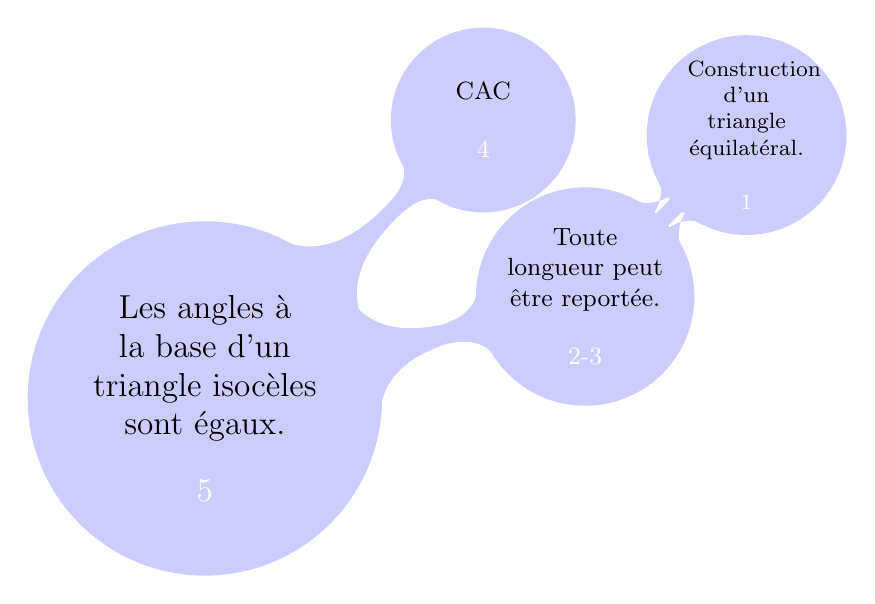
\begin{tikzpicture}
    [root concept/.append style={concept color=blue!20},
    level 1 concept/.append style={sibling angle=30},
    mindmap]
    \node [concept] {Les angles à la base d'un triangle isocèles sont égaux.\vskip10pt
    {\color{white}5}}
    [clockwise from=45]
    child { node[concept] (c1) {CAC\vskip10pt\color{white}4}}
    child { node[concept] (c2) {Toute longueur peut être reportée.\vskip10pt\color{white}2-3}
        child{node[concept] {Construction d'un triangle équilatéral.\vskip10pt\color{white}1}}
    };
    
\end{tikzpicture}    

\end{document}
